\documentclass[10pt, twocolumn]{article}
\usepackage[utf8]{inputenc}
\usepackage[fleqn]{amsmath}
\usepackage[]{fullpage}
\usepackage[]{times}
\usepackage[]{graphicx}
\linespread{0.75}
\title{Homework 1: Review of Prerequisites}
\author{Rahul Krishna}
\date{}
\setlength{\mathindent}{0cm}
\setlength{\parindent}{0cm}
\setlength{\parskip}{0em}
\setlength{\lineskip}{0em}
\newcommand{\bml}{\begin{multline}}
\newcommand{\eml}{\end{multline}\\[-0.5cm]}
\newcommand{\bbml}{\begin{multline*}}
\newcommand{\eeml}{\end{multline*}\\[-0.5cm]}

% \renewcommand{\baselinestretch}{0.1}

\begin{document}

\maketitle
\subsection*{1}
\textbf{a.}
\begin{multline*}
\text{At $n=4$ we have,}\\
4!=24 \text{ and } 2^4=16 \\
\text{Thus, }4!\ge2^4\\
\text{Likewise, at n=10: }\\
10!=3628800 \text{ and } 2^{10}=1024 \\
\text{Thus, }10!\ge10^4\hfill\\
\text{Now, lets assume this holds true at } n=k.\\
\text{Thus, }k!\ge2^k\hfill\\
\text{Now, at k+1: }\\
( k+1! )=(k+1)\times(k!)\\
2^{k+1} = 2\times2^k\\
\text{We know from (1) that }k!\ge2^k\\\text{And }k+1>2\text{ since, }k\ge4\\
\text{We get }(k+1)!\ge2^{k+1}\\
\text{Thus, using mathematical induction we can prove that }\\n!\ge2^n\text{ for }n\ge4\hfill
\end{multline*}
\textbf{b.\\[-0.25cm]}
\begin{multline*}
\text{At $n=2$, we have }\\
2^3-2=6\text{, and this is divisible by 3.}\\
\text{Now, let's assume that this is true at n=k. Thus,}\\
f(k)=k^3-k\text{ is divisible by 3.}\hfill(1)\\
\text{Now, at n=k+1, we have,}\\
f(k+1)=(k+1)^3-(k+1), \text{solving for this,}\\
f(k+1)=k^3+1+3+3k-k-1\\
f(k+1)=k^3+2k+3\\
f(k+1)=k^3-k+3k+3=f(k)+3\times(k+1)\hfill(2)\\[0.2cm]
\text{Now, we know from (1) that $f(k)$ is divisible by 3, }\\
\text{and so is } 3\times(k+1)\hfill\\[0.2cm]
\text{Thus, using mathematical induction we can prove that }\\n^3-n\text{ is divisible by 3 for }n\ge0\hfill
\end{multline*}
\vfill
\subsection*{2}
\textbf{a.\\[-0.25cm]}
\begin{multline*}
f(n) = \sum\limits_{i = 0}^n {{{\left( {\frac{{i + 1}}{2}} \right)}^2}}\hfill\\
f(n) = \tfrac{1}{4}\sum\limits_{i = 0}^n {{i^2}}  + \tfrac{1}{4}\sum\limits_{i = 0}^n 1  + \tfrac{1}{2}\sum\limits_{i = 0}^n i\hfill\\
f(n) = \\\frac{1}{4}\left( {\frac{1}{6}n\left( {n + 1} \right)\left( {2n + 1} \right)} \right) + \frac{1}{2}\left( {\frac{1}{2}n\left( {n + 1} \right)} \right) + \frac{1}{4}\left( {n + 1} \right)\\\\
f(n) = \frac{1}{4}\left( {n + 1} \right)\left( {\frac{1}{6}n\left( {2n + 1} \right) + \frac{n}{4} + 1} \right)
\end{multline*}

\textbf{b.\\[-0.25cm]}
\begin{multline*}
f(n) = \sum\limits_{i = 0}^n {{4^i}{7^{n - i}}}={7^n}\sum\limits_{i = 0}^n {{{\left( {\tfrac{4}{7}} \right)}^i}}\hfill\\
f(n) = {7^n} \times \frac{7}{3}\left( {1 - \frac{{{4^{n + 1}}}}{{{7^{n + 1}}}}} \right) = \frac{1}{3}\left( {{7^{n + 1}} - {4^{n + 1}}} \right)\hfill\\
\end{multline*}

\subsection*{3}
\textbf{Original Statement:} \textit{Every planar graph can be coloured with four colours.}\\

\textbf{a. Contrapositive Statement:} \textit{If a graph cannot be coloured with four colours then it is not a planar graph.}\\

\textbf{a. Converse Statement:} \textit{If a graph can be coloured with four colours then it is a planar graph.}\\

\subsection*{4}
\[A_{n\times n} = \begin{array}{*{20}{c}}
  {{i \mathord{\left/
 {\vphantom {i j}} \right.
 \kern-\nulldelimiterspace} j}}&{\begin{array}{*{20}{c}}
  1&2& \cdots & \cdots &n 
\end{array}} \\ 
  {\begin{array}{*{20}{c}}
  1 \\ 
  2 \\ 
   \vdots  \\ 
   \vdots  \\ 
  n 
\end{array}}&{\left[ {\begin{array}{*{20}{c}}
  2&0&0&0&0 \\ 
  1&2&0&0&0 \\ 
   \vdots & \vdots & \ddots & \vdots & \vdots  \\ 
   \vdots & \vdots & \ldots & \vdots & \vdots  \\ 
  1&1&1&1&2 
\end{array}} \right]} 
\end{array}\]


\textbf{a.\\[0.25cm]}
Since this is a triangular matrix (a lower triangular matrix to be precise), the determinant of this matrix is the product of all the diagonal elements. Thus, \[\left| A_{n\times n} \right| = {2^n}\]

\textbf{b. \\[0.25cm]}
Since the determinant of $A$ is non-zero, an inverse can be computed. To do so, we may use the Gauss-Jordan elimination method. Let's start with  $A_{3\times 3}$.
\[{A_{3 \times 3}} = \left[ {\left. {\begin{array}{*{20}{c}}
  2&0&0 \\ 
  1&2&0 \\ 
  1&1&2 
\end{array}} \right|\begin{array}{*{20}{c}}
  1&0&0 \\ 
  0&1&0 \\ 
  0&0&1 
\end{array}} \right]\]

\[\begin{array}{*{20}{c}}
  {\left[ {\left. {\begin{array}{*{20}{c}}
  2&0&0 \\ 
  1&2&0 \\ 
  1&1&2 
\end{array}} \right|\begin{array}{*{20}{c}}
  1&0&0 \\ 
  0&1&0 \\ 
  0&0&1 
\end{array}} \right]} \\[0.5cm] 
{ \downarrow {\begin{array}{*{20}{c}}
  {{R_2} = {R_2} - \tfrac{1}{2}{R_1}} \\ 
  {{R_3} = {R_3} - \tfrac{1}{2}{R_1}} 
\end{array}}} \\[0.35cm] 
  {\left[ {\left. {\begin{array}{*{20}{c}}
  2&0&0 \\ 
  0&2&0 \\ 
  0&1&2 
\end{array}} \right|\begin{array}{*{20}{c}}
  1&0&0 \\ 
  { - {\raise0.5ex\hbox{$\scriptstyle 1$}
\kern-0.1em/\kern-0.15em
\lower0.25ex\hbox{$\scriptstyle 2$}}}&1&0 \\ 
  { - {\raise0.5ex\hbox{$\scriptstyle 1$}
\kern-0.1em/\kern-0.15em
\lower0.25ex\hbox{$\scriptstyle 2$}}}&0&1 
\end{array}} \right]} \\[0.5cm]
  { \downarrow \tiny{{R_3} = {R_3} - \tfrac{1}{2}{R_2}}} \\[0.25cm]
  {\left[ {\left. {\begin{array}{*{20}{c}}
  2&0&0 \\ 
  0&2&0 \\ 
  0&0&2 
\end{array}} \right|\begin{array}{*{20}{c}}
  1&0&0 \\ 
  { - {\raise0.5ex\hbox{$\scriptstyle 1$}
\kern-0.1em/\kern-0.15em
\lower0.25ex\hbox{$\scriptstyle 2$}}}&1&0 \\ 
  { - {\raise0.5ex\hbox{$\scriptstyle 1$}
\kern-0.1em/\kern-0.15em
\lower0.25ex\hbox{$\scriptstyle 2$}}}&{ - {\raise0.5ex\hbox{$\scriptstyle 1$}
\kern-0.1em/\kern-0.15em
\lower0.25ex\hbox{$\scriptstyle 2$}}}&1 
\end{array}} \right]} \\[0.5cm] 
  {\begin{array}{*{20}{c}}
  { \downarrow \begin{array}{*{20}{c}}
  {{R_1} = \tfrac{1}{2}{R_1}} \\ 
  {{R_2} = \tfrac{1}{2}{R_2}} \\ 
  {{R_3} = \tfrac{1}{2}{R_3}} 
\end{array}}&{} 
\end{array}} \\[0.65cm] 
  {\left[ {\left. {\begin{array}{*{20}{c}}
  1&0&0 \\ 
  0&1&0 \\ 
  0&0&1 
\end{array}} \right|\begin{array}{*{20}{c}}
    { - {\raise0.5ex\hbox{$\scriptstyle 1$}
\kern-0.1em/\kern-0.15em
\lower0.25ex\hbox{$\scriptstyle 2$}}}&0&0 \\ 
  { - {\raise0.5ex\hbox{$\scriptstyle 1$}
\kern-0.1em/\kern-0.15em
\lower0.25ex\hbox{$\scriptstyle 4$}}}&{ - {\raise0.5ex\hbox{$\scriptstyle 1$}
\kern-0.1em/\kern-0.15em
\lower0.25ex\hbox{$\scriptstyle 2$}}}&0 \\ 
  { - {\raise0.5ex\hbox{$\scriptstyle 1$}
\kern-0.1em/\kern-0.15em
\lower0.25ex\hbox{$\scriptstyle 8$}}}&{ - {\raise0.5ex\hbox{$\scriptstyle 1$}
\kern-0.1em/\kern-0.15em
\lower0.25ex\hbox{$\scriptstyle 4$}}}&{ - {\raise0.5ex\hbox{$\scriptstyle 1$}
\kern-0.1em/\kern-0.15em
\lower0.25ex\hbox{$\scriptstyle 2$}}} 
\end{array}} \right]}\\[0.5cm] 
\end{array}\]

Thus,

\[A{{}_{3 \times 3}^{ - 1}} = \left[\begin{array}{*{20}{c}}
    { - {\raise0.5ex\hbox{$\scriptstyle 1$}
\kern-0.1em/\kern-0.15em
\lower0.25ex\hbox{$\scriptstyle 2$}}}&0&0 \\ 
  { - {\raise0.5ex\hbox{$\scriptstyle 1$}
\kern-0.1em/\kern-0.15em
\lower0.25ex\hbox{$\scriptstyle 4$}}}&{ - {\raise0.5ex\hbox{$\scriptstyle 1$}
\kern-0.1em/\kern-0.15em
\lower0.25ex\hbox{$\scriptstyle 2$}}}&0 \\ 
  { - {\raise0.5ex\hbox{$\scriptstyle 1$}
\kern-0.1em/\kern-0.15em
\lower0.25ex\hbox{$\scriptstyle 8$}}}&{ - {\raise0.5ex\hbox{$\scriptstyle 1$}
\kern-0.1em/\kern-0.15em
\lower0.25ex\hbox{$\scriptstyle 4$}}}&{ - {\raise0.5ex\hbox{$\scriptstyle 1$}
\kern-0.1em/\kern-0.15em
\lower0.25ex\hbox{$\scriptstyle 2$}}} 
\end{array} \right]\]

Similarly, for $A_{5\times 5}$, we get

\[A_{5 \times 5}^{ - 1} = \left[ {\begin{array}{*{20}{c}}
  {{2^{ - 1}}}&0&0&0&0 \\ 
  {{2^{ - 2}}}&{{2^{ - 1}}}&0&0&0 \\ 
  {{2^{ - 3}}}&{{2^{ - 2}}}&{{2^{ - 1}}}&0&0 \\ 
  {{2^{ - 4}}}&{{2^{ - 3}}}&{{2^{ - 2}}}&{{2^{ - 1}}}&0 \\ 
  {{2^{ - 5}}}&{{2^{ - 4}}}&{{2^{ - 3}}}&{{2^{ - 2}}}&{{2^{ - 1}}} 
\end{array}} \right]\]

This procedure can be extended to $A_{n\times n}$ to obtain,

\[A_{n \times n}^{ - 1} = \left[ {\begin{array}{*{20}{c}}
  {{2^{ - 1}}}&0& \cdots &0&0 \\ 
  {{2^{ - 2}}}&{{2^{ - 1}}}& \cdots &0&0 \\ 
   \vdots & \vdots & \ddots & \vdots & \vdots  \\ 
  {{2^{ - (n - 1)}}}&{{2^{ - (n - 2)}}}& \cdots &{{2^{ - 1}}}&0 \\ 
  {{2^{ - n}}}&{{2^{ - (n - 1)}}}& \cdots &{{2^{ - 2}}}&{{2^{ - 1}}} 
\end{array}} \right]\]

\textbf{c. \\[0.25cm]}
\[A_{n \times n}^T = \left[ {\begin{array}{*{20}{c}}
  2&1& \cdots &1&1 \\ 
  2&1& \cdots &1&1 \\ 
   \vdots & \vdots & \ddots & \vdots & \vdots  \\ 
  0&0& \cdots &2&1 \\ 
  0&0& \cdots &0&2 
\end{array}} \right]\]

\subsection*{6}
\[{a_{n}} = 3{a_{n - 1}} - {a_{n - 2}}\]
\[{a_{n}} - 3{a_{n - 1}} + {a_{n - 2}} = 0\hfill(1)\]
The characteristic equation of $(1)$ is given by,
\[{x^2} - 3x + 1 = 0\]
Solving above,
\[x = \tfrac{1}{2}\left( {3 + \sqrt 5 } \right),\tfrac{1}{2}\left( {3 - \sqrt 5 } \right)\]
Thus, $a_n$ can be represented as below,
\[{a_n} = {c_1} \times {\left[ {\tfrac{1}{2}\left( {3 + \sqrt 5 } \right)} \right]^n} + {c_2} \times {\left[ {\tfrac{1}{2}\left( {3 - \sqrt 5 } \right)} \right]^n}\]
Where $c_1$ and $c_2$ are arbitrary constants. At, n=0
\[c_1+c_2=0\hfill(2)\]
\text{And at, }n=1
\[{c_1}  {\left[ {\tfrac{1}{2}\left( {3 + \sqrt 5 } \right)} \right]} + {c_2}  {\left[ {\tfrac{1}{2}\left( {3 - \sqrt 5 } \right)} \right]}=1\hfill(3)\]
Solving $(2)$ and $(3)$, we get
\[{c_1} = {\raise0.7ex\hbox{$1$} \!\mathord{\left/
 {\vphantom {1 {\sqrt 5 }}}\right.\kern-\nulldelimiterspace}
\!\lower0.7ex\hbox{${\sqrt 5 }$}}\\
{c_2} =  - {\raise0.7ex\hbox{$1$} \!\mathord{\left/
 {\vphantom {1 {\sqrt 5 }}}\right.\kern-\nulldelimiterspace}
\!\lower0.7ex\hbox{${\sqrt 5 }$}}\]
Thus,
\[{a_n} = {\raise0.7ex\hbox{$1$} \!\mathord{\left/
 {\vphantom {1 {\sqrt 5 }}}\right.\kern-\nulldelimiterspace}
\!\lower0.7ex\hbox{${\sqrt 5 }$}}{\left[ {\tfrac{1}{2}\left( {3 + \sqrt 5 } \right)} \right]^n} - {\raise0.7ex\hbox{$1$} \!\mathord{\left/
 {\vphantom {1 {\sqrt 5 }}}\right.\kern-\nulldelimiterspace}
\!\lower0.7ex\hbox{${\sqrt 5 }$}}{\left[ {\tfrac{1}{2}\left( {3 - \sqrt 5 } \right)} \right]^n}\]
\subsection*{7}
\textit{"Every vertex transitive graph does not necessarily have a Hamiltonian path."}
\subsection*{8}
\textbf{a. } $n$ is a positive integer, the smallest n is $n=1$. Therefore, the smallest counterexample is $n=1$. Because, at the value of n, there are no positive integer values of a and b that satisfy the relation $n=2a+9b$.\\

\textbf{b. } The Largest counter example is 18. AT $b=1$ and $a=4$ we get $n=17$ and the next valid value of $n$ is $19$ and beyond this, the conjecture holds true of all positive integer values of $n$.\\

\textbf{c. } \textit{Theorem: For all integers $n\ge19$, there exist positive integers $a$ and $b$ such that $n=2a+9b$.}
\newpage
\subsection*{5}
\textbf{a. }
\begin{figure}[h]
    \centering
    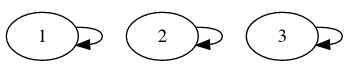
\includegraphics[width=0.99\linewidth]{i8_1.png}
    \caption{$G_1$}
    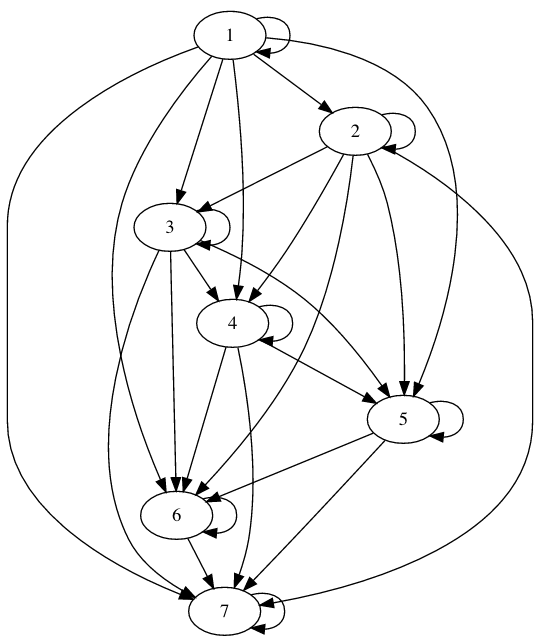
\includegraphics[width=1\linewidth]{i8_2.png}
    \caption{$G_2$}
    \label{fig:my_label}
\end{figure}

\textbf{b. } Number of vertices$=2k+1$\\

\textbf{c. } Number of edges$={(2k+1)(k+1)}$

\end{document}
